
\section{Эксперимент BM@N (NICA)}

\subsection{Ускорительный комплекс NUCLOTRON-NICA}

Эксперимент BM@N располагается на выведенном пучке ускорителя NUCLOTRON, который является частью ускорительного комплеса NICA, ОИЯИ, Дубна.
Линейный ускоритель тяжелых ионов Linac инжектирует пучок в кольцевой ускоритель Boster.
После ускорения тяжелых ионов в кольце Booster до энергии в $0.5A$~ГэВ, пучок подаётся на NUCLOTRON.
Максимальные энергии, достижимые Nuclotron составляют до $4.5A$~ГэВ.
После ускорения ядер до необходимой энергии, пучок может быть отправлен как на эксперимент BM@N, так и на коллайдер NICA.

\subsection{Схема установки}

BM@N является экспериментом с фиксированной мишенью.
Схема экспериментальной установки представлена на рис.~\ref{fig:bmn_layout}.
Далее будут рассмотрены основные подсистемы спектрометра, информация с которых была использована для анализа.
%
\begin{figure}[ht]
\begin{center}
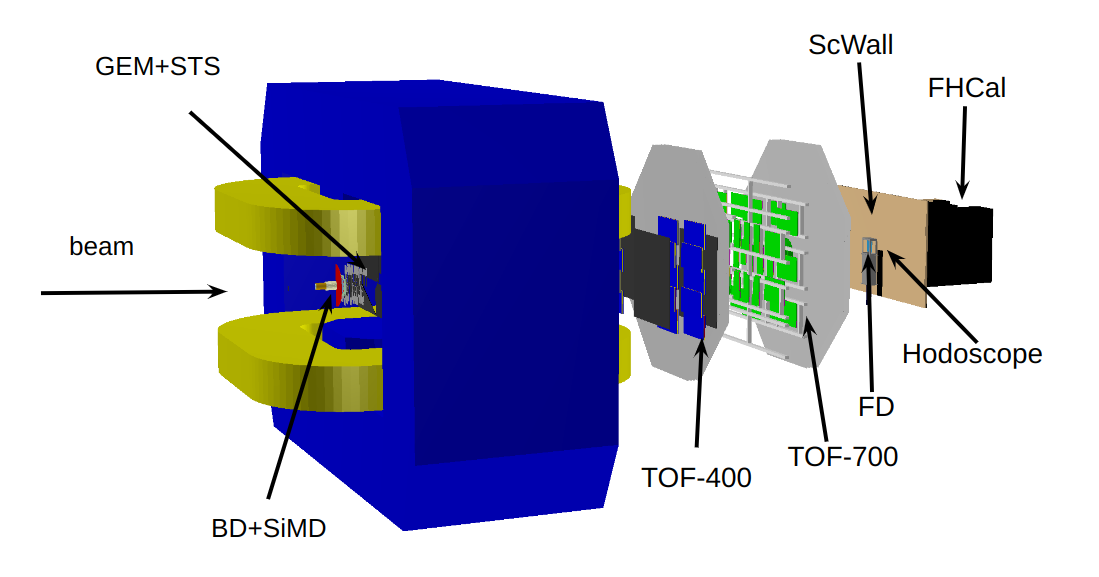
\includegraphics[width=0.95\linewidth]{images/BM@N_layout.png}
\caption{Схема эксперимента BM@N.}
\label{fig:bmn_layout}
\end{center}
\end{figure}

\subsection{Трекинговая система}

Система реконструкции траекторий заряженных частиц в эксперименте BM@N состоит из четырех станций кремниевых детекторов (Forward Silicon Detector, FSD) и семи станций газо-электронных умножителей (GEM). 
В отличие от HADES, трекинговая система целиком находится в магнитном поле дипольного магнита что позволяет с большой точностью восстанавливать импульсы рожденных в столкновении заряженных частиц.
На рис.~\ref{fig:bmn_tracking} представлено схематическое изображение трекинговой системы в эксперименте BM@N.
Траектории заряженных частиц отклоняются магнитным полем дипольного магнита, что позволяет восстанавливать импульс заряженных частиц.
Вакуумная пучковая труба позволяет минимизировать столкновения ядер цезия с атомами азота, кислорода и прочими примесями.
Поскольку вакуумная труба также расположена в магнитном поле, она имеет искривлённую форму для свободного прохождения невзаимодействоваших ядер пучка.  
%
\begin{figure}[ht]
\begin{center}
    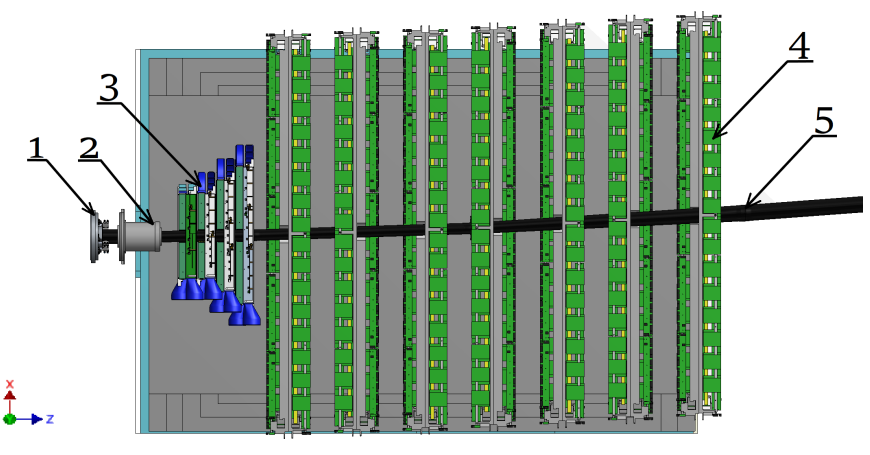
\includegraphics[width=0.75\linewidth]{images/bmn_tracking_system.png}
    \caption{Схематическое изображение трекинговой системы в эксперименте BM@N. Цифрами (1) обозначена мишень,
    (2) --- Barell Detector, (3) --- FSD, (4) --- GEM, (5) --- Beam Pipe }
    \label{fig:bmn_tracking}
\end{center}
\end{figure}

Центральная система трекинга (CTS) состоит из двух основных систем детекторов: детектора кремниевого фронта (FSD) и набора газовых электронных умножителей (GEM). 
Эти системы расположены внутри анализирующего магнита SP-41. 
FSD расположен непосредственно за областью мишени, в то время как GEM-детекторы установлены вниз по течению, внутри межполюсного объема.

FSD состоит из четырех плоскостей трекинга, каждая из которых разделена на две полуплоскости. 
Полуплоскости изготовлены из координатных модулей на основе DSSD, электронной кросс-платы, подвески и механики точного позиционирования, кабельного коммутационного блока, воздушного охлаждения, мониторов температуры и светового и электромагнитного экрана. 
Конструкция допускает вертикальное перемещение полуплоскостей во время сборки и перекрытие активных областей в рабочем положении. 
В центре каждой плоскости имеется нечувствительная зона размером 57 × 57 мм2 для размещения трубы пучка.

Каждая плоскость FSD содержит несколько модулей, оснащенных детекторами DSSD. 
Детекторы DSSD изготовлены из кремниевых пластин с высоким удельным сопротивлением и имеют полосы с обеих сторон. 
Полосы соединены методом US-склеивания и имеют шаг 95 и 103 мкм. 
Детекторы расположены таким образом, что полосы стороны p + выровнены с осью Y.

Электроника считывания для FSD включает в себя интегральные схемы PA-640, которые выполняют функции смещения и согласования. 
Сигналы от DSSD затем подаются на ASIC VATAGP7.1, которые усиливают, формируют и хранят импульсы. 
ASIC монтируются на печатных платах и подключаются к адаптерам шага.

Система трекинга GEM состоит из семи плоскостей трекинга, каждая из которых имеет верхний и нижний детектор. 
Детекторы изготавливаются с использованием технологии "фольги-растяжения" без клея и имеют три фольги GEM с перфорированными отверстиями. 
Катод изготовлен из фольги Каптона, покрытой медью, а анодная плоскость используется для считывания. 
Плоскость считывания разделена на две половины и имеет "горячую зону" для более высокой плотности попаданий.
GEM-детекторы работают при высоком напряжении и имеют определенные электрические поля в зазорах между электродами. 

\subsection{Времяпролётные детекторы TOF-400 и TOF-700}

Эксперимент BM@N использует две системы времени пролета (TOF), TOF400 и TOF700, для идентификации заряженных частиц. 
TOF400 расположен на расстоянии 4 метра от мишени и состоит из двух плеч с детекторами MRPC. 
TOF700 расположен на расстоянии 7 метров от мишени и имеет большую активную область. 
Обе системы перекрываются с другими детекторами и обеспечивают непрерывный геометрический аксептанс.

Выбор детекторов MRPC для TOF был основан на их высокой гранулярности, скорости, позиционном разрешении, эффективности и возможностях разделения частиц. 
Система TOF400 имеет более высокий поток частиц, чем система TOF700.

Система TOF400 состоит из двух плеч с модулями MRPC. 
Каждый модуль имеет пять детекторов MRPC с активной площадью 60 × 30 см². 
Детекторы расположены таким образом, чтобы обеспечивать перекрытие активных областей. 
Газовые коробки для системы TOF400 изготовлены из алюминиевых рам и сотовых панелей. 
MRPC в системе TOF400 имеют конструкцию стопки со стеклянными пластинами и плоскостью считывания. 
Электроника считывания для TOF400 использует ASIC NINO и аналого-цифровые преобразователи времени TDC72VHL.

Система TOF700 состоит из "холодных" и "теплых" детекторов MRPC. "Холодные" MRPC имеют большую активную область и меньше считывающих полос, чем "теплые" MRPC. 
MRPC в системе TOF700 расположены в два слоя и имеют другую конструкцию с уменьшенными газовыми зазорами и толщиной стеклянных пластин. 
Электроника считывания для TOF700 также основана на ASIC NINO и аналого-цифровых преобразователях времени TDC72VHL.

Обе системы TOF используют одинаковую газовую смесь и имеют схожие условия работы. 
Системы питания высокого напряжения для обеих подсистем TOF основаны на коммерчески доступных модулях Iseg.

На рис.~\ref{fig:bmn_beta_pq} показано распределение заряженных частиц по относительной скорости $\beta=v/c$ и импульсу деленному на заряд $p/q$.
%
\begin{figure}[ht]
\begin{center}
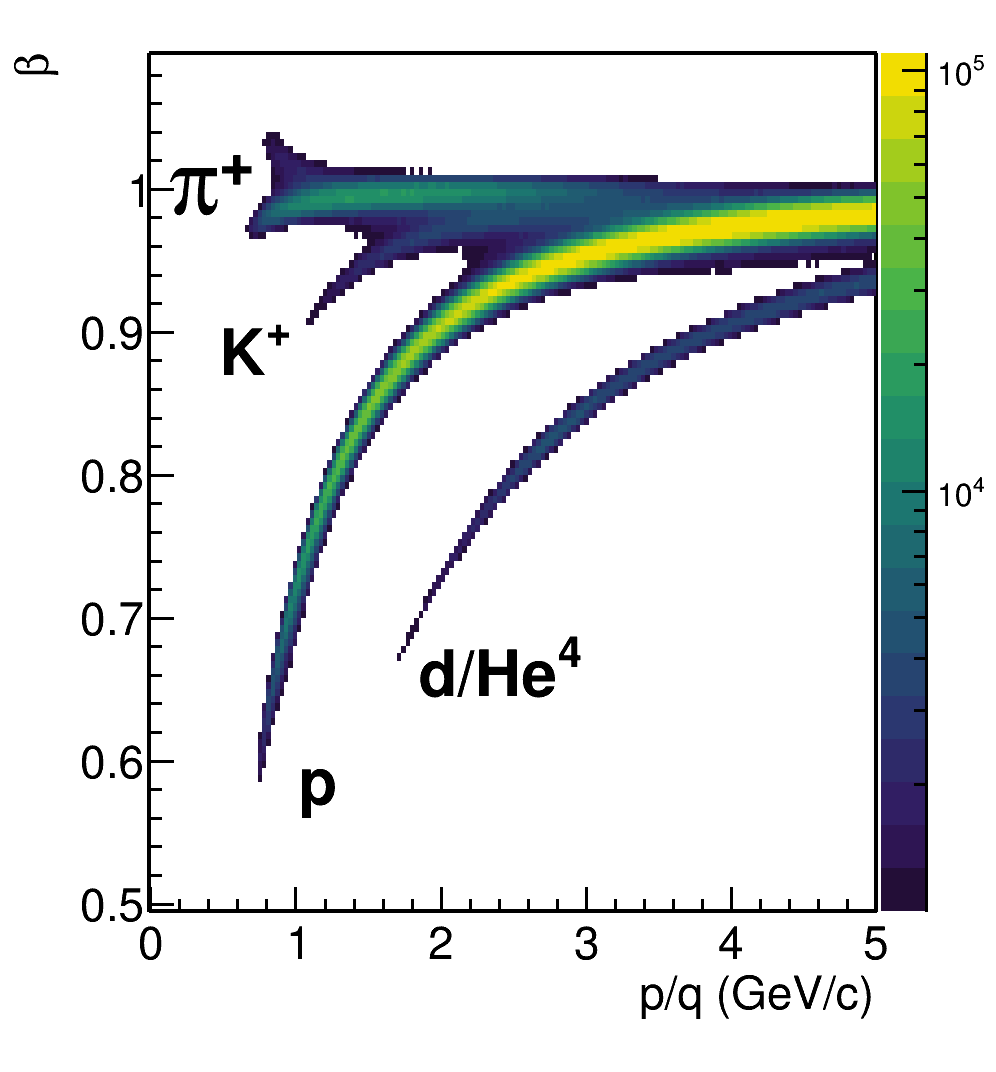
\includegraphics[width=0.55\linewidth]{images/beta_pq.png}
\caption{Распределение заряженных частиц по относительной скорости $\beta=v/c$ и импульсу деленному на заряд $p/q$.}
\label{fig:bmn_beta_pq}
\end{center}
\end{figure}

\subsection{Передний адронный калориметр FHCal}

Передний Адронный калориметр (FHCal) в эксперименте BM@N является сэмплирующим калориметром, предназначенным для измерения энергии адронов и других частиц, образующихся в столкновениях тяжелых ионов. 
Он состоит из 54 отдельных модулей, расположенных в поперечной плоскости. 
Внутренняя часть FHCal состоит из 34 небольших модулей с поперечными размерами 15 × 15 см² и длиной, эквивалентной 4,0 ядерным длинам взаимодействия. 
Эти модули идентичны модулям переднего адронного калориметра многоцелевого детектора (MPD) в ускорительном комплексе NICA. 
Две внешне-боковые части калориметра содержат 10 более крупных модулей с поперечным размером 20 × 20 см² и длиной, эквивалентной 5,6 ядерным длинам взаимодействия. 
Эти модули первоначально были построены для адронного калориметра эксперимента по сжатой барионной материи (CBM) (FAIR, Дармштадт, Германия) и временно используются в эксперименте BM@N.

Модули FHCal имеют сэмплирующую структуру и состоят из слоев свинца/сцинтиллятора с отношением сэмплирования 4:1. 
Небольшие модули имеют 42 слоя свинца/сцинтиллятора, в то время как большие модули имеют 60 таких слоев. 
Сцинтилляционные пластины изготовлены из пластикового сцинтиллятора на основе полистирола и собирают свет с помощью оптических волокон. 
Свет транспортируется до конца модуля и считывается фотодетекторами.
Энергетическое разрешение FHCal составляет 0,54/ √ E.
Схема расположения модулей калориметра представлена на рис.~\ref{fig:fhcal_layout} справа.
%
\begin{figure}[ht]
\begin{center}
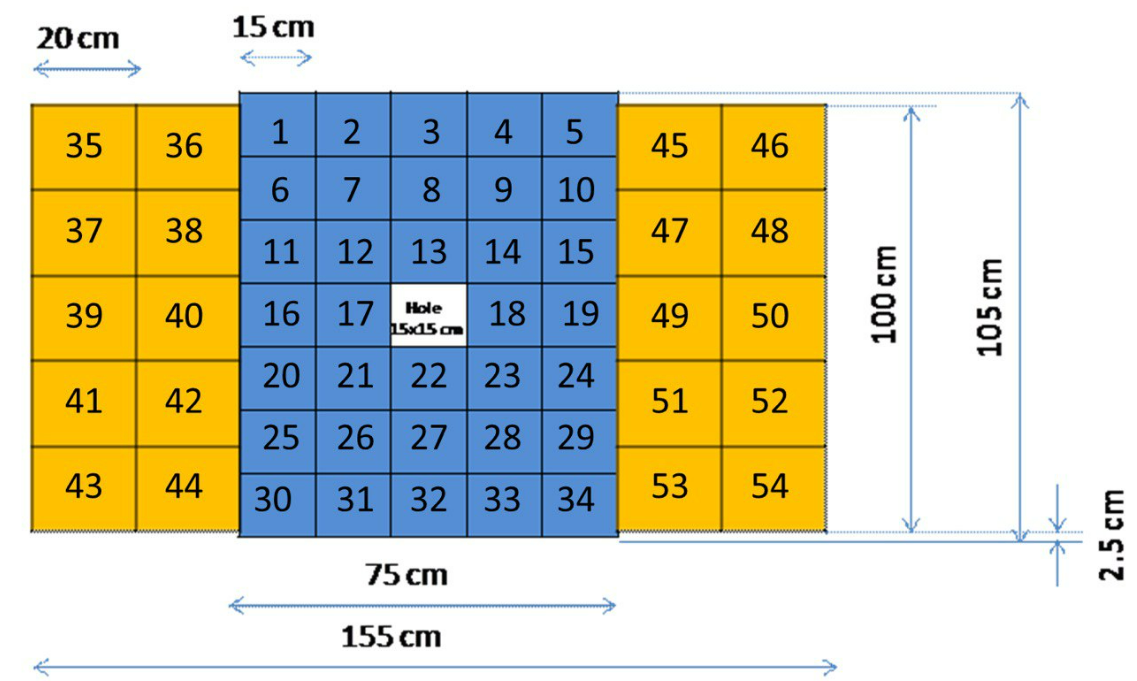
\includegraphics[width=0.55\linewidth]{images/FHCal_modules.png}
\caption{Схема расположения модулей переднего адронного калориметра FHCal.}
\label{fig:fhcal_layout}
\end{center}
\end{figure}

\section{Выводы к главе 2}

В главе описывается устройство экспериментальной установки HADES. 
Рассмотрены принципы работы основных детекторных подсистем, таких как трекинговая система, триггерная система, времяпролётная система и передний годоскоп Forward Wall.
В главе приведено краткое описание установки BM@N и ее детекторов.
Рассмотрены принципы работы трекинговой системы, описано устройство времяпролётной системы и переднего адронного калориметра FHCal.
